\documentclass{standalone}

\usepackage[OT1]{fontenc}
\renewcommand*\familydefault{\sfdefault}
\usepackage{helvet,sfmath}
\usepackage{siunitx}

\usepackage{tikz}
\usetikzlibrary{arrows,calc,patterns}
\usepackage{tikz,tkz-euclide}

\definecolor{BlueDefault}{rgb}{0.2,0.2,0.7}

\begin{document}

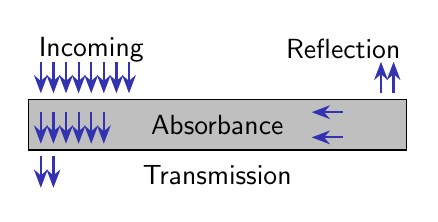
\begin{tikzpicture}[scale=0.8]
    \draw[fill = lightgray] (-3,-0.4) to (-3,0.4) to (3,0.4) to (3,-0.4) to (-3,-0.4);
    \draw 
    (0,0) node{Absorbance}
    (-2,1.2) node{Incoming}
    (2,1.2) node{Reflection}
    (0,-0.8) node{Transmission}
    ;
    %%Incoming wave
    \draw[BlueDefault, thick, -Stealth] (-2.8,1) to (-2.8,0.5);
    \draw[BlueDefault, thick, -Stealth] (-2.6,1) to (-2.6,0.5);
    \draw[BlueDefault, thick, -Stealth] (-2.4,1) to (-2.4,0.5);
    \draw[BlueDefault, thick, -Stealth] (-2.2,1) to (-2.2,0.5);
    \draw[BlueDefault, thick, -Stealth] (-2.0,1) to (-2.0,0.5);
    \draw[BlueDefault, thick, -Stealth] (-1.8,1) to (-1.8,0.5);
    \draw[BlueDefault, thick, -Stealth] (-1.6,1) to (-1.6,0.5);
    \draw[BlueDefault, thick, -Stealth] (-1.4,1) to (-1.4,0.5);
    %%Wave in matter
    \draw[BlueDefault, thick, -Stealth] (-2.8,0.2) to (-2.8,-0.3);
    \draw[BlueDefault, thick, -Stealth] (-2.6,0.2) to (-2.6,-0.3);
    \draw[BlueDefault, thick, -Stealth] (-2.4,0.2) to (-2.4,-0.3);
    \draw[BlueDefault, thick, -Stealth] (-2.2,0.2) to (-2.2,-0.3);
    \draw[BlueDefault, thick, -Stealth] (-2.0,0.2) to (-2.0,-0.3);
    \draw[BlueDefault, thick, -Stealth] (-1.8,0.2) to (-1.8,-0.3);
    %Reflection wave
    \draw[BlueDefault, thick, -Stealth] (2.8,0.5) to (2.8,1);
    \draw[BlueDefault, thick, -Stealth] (2.6,0.5) to (2.6,1);
    %%Transission wave
    \draw[BlueDefault, thick, -Stealth] (-2.8,-0.5) to (-2.8,-1);
    \draw[BlueDefault, thick, -Stealth] (-2.6,-0.5) to (-2.6,-1);
    %%Absorbance
    \draw[BlueDefault, thick, -Stealth] (2.0,0.2) to (1.5,0.2);
    \draw[BlueDefault, thick, -Stealth] (2.0,-0.2) to (1.5,-0.2);
\end{tikzpicture}

\end{document}